%% Lab Report for EEET2493_labreport_template.tex
%% V1.0
%% 2019/01/16
%% This is the template for a Lab report following an IEEE paper. Modified by Francisco Tovar after Michael Sheel original document.


%% This is a skeleton file demonstrating the use of IEEEtran.cls
%% (requires IEEEtran.cls version 1.8b or later) with an IEEE
%% journal paper.
%%
%% Support sites:
%% http://www.michaelshell.org/tex/ieeetran/
%% http://www.ctan.org/pkg/ieeetran
%% and
%% http://www.ieee.org/

%%*************************************************************************
%% Legal Notice:
%% This code is offered as-is without any warranty either expressed or
%% implied; without even the implied warranty of MERCHANTABILITY or
%% FITNESS FOR A PARTICULAR PURPOSE! 
%% User assumes all risk.
%% In no event shall the IEEE or any contributor to this code be liable for
%% any damages or losses, including, but not limited to, incidental,
%% consequential, or any other damages, resulting from the use or misuse
%% of any information contained here.
%%
%% All comments are the opinions of their respective authors and are not
%% necessarily endorsed by the IEEE.
%%
%% This work is distributed under the LaTeX Project Public License (LPPL)
%% ( http://www.latex-project.org/ ) version 1.3, and may be freely used,
%% distributed and modified. A copy of the LPPL, version 1.3, is included
%% in the base LaTeX documentation of all distributions of LaTeX released
%% 2003/12/01 or later.
%% Retain all contribution notices and credits.
%% ** Modified files should be clearly indicated as such, including  **
%% ** renaming them and changing author support contact information. **
%%*************************************************************************

\documentclass[journal]{IEEEtran}

% *** CITATION PACKAGES ***
\usepackage[style=ieee]{biblatex} 
\bibliography{example_bib.bib}    %your file created using JabRef
\usepackage{hyperref}
% *** MATH PACKAGES ***
\usepackage{amsmath}
 \usepackage{multirow}

% *** PDF, URL AND HYPERLINK PACKAGES ***
\usepackage{url}
% correct bad hyphenation here
\hyphenation{op-tical net-works semi-conduc-tor}
\usepackage{graphicx}  %needed to include png, eps figures
\usepackage{float}  % used to fix location of images i.e.\begin{figure}[H]

\begin{document}

% paper title
\title{Guidelines for a Lab report 3 EEET2493 \\
\small{Title of the session (you can be creative highlighting your findings)}}

% author names 
\author{Student name 1, s123456,
        Student name 2, s123456,
        Student name 3, s123456,
        {\small Names are to be centered in Times 
(or Times Roman) 12-point nonboldface. Leave two blank lines before your Abstract}}% <-this % stops a space
        
% The report headers
\markboth{EEET2493 Biomedical Instrumentation. Lab. Report 3. May 2019    \quad   \quad \quad \quad   \quad \quad \quad  \quad   \quad \quad \quad   \quad \quad TOTAL: 10 MARKS}%do not delete next lines
{Shell \MakeLowercase{\textit{et al.}}: Bare Demo of IEEEtran.cls for IEEE Journals}

% make the title area
\maketitle

% As a general rule, do not put math, special symbols or citations
% in the abstract or keywords.
\begin{flushright} Title and abstract: 1 marks. \end{flushright}
\begin{abstract} Provide a summary of the session. What was done, 
what measurements were taken, brief methods, what calculations, brief conclusion.  The Abstract should be approximately 250 words or fewer, italicized, in 10-point Times (or Times Roman.) Please leave two spaces between the Abstract and the heading of your first section.
It should briefly summarize the essence of the paper and address the following areas without using specific subsection titles. Objective: Briefly state the problem or issue addressed, in language accessible to a general scientific audience. Technology or Method: Briefly summarize the technological innovation or method used to address the problem. Results: Provide a brief summary of the results and findings. Conclusions: Give brief concluding remarks on your outcomes. Detailed discussion of these aspects should be provided in the main body of the paper. 
\end{abstract}

\begin{IEEEkeywords}
keywords, temperature, xxxx equation, etc.
\end{IEEEkeywords}

\section{Introduction   }
\begin{flushright} 1.2 Marks \end{flushright}

% Here we have the typical use of a "W" for an initial drop letter
% and "RITE" in caps to complete the first word.
% You must have at least 2 lines in the paragraph with the drop letter
% (should never be an issue)

\IEEEPARstart{D}{escribe:} Why is important to design instruments with reliable data output and user-friendly for biomedical engineering?  (1 paragraph 3-5 lines. 0.2 marks).\\[0.1in] 
How the integration of a microcontroler into instrument's design  contributes to the idea developed in the last paragraph? (1 paragraph 3-5 lines. 0.2 marks).\\[0.1in] 
What are the most common measurands in biomedical engineering that are possible to obtain with the use of appropriate sensors and micro-controllers? (1 paragraph 3-5 lines. 0.2 marks).\\[0.15in] 
Why is important to measure force in biomedical engineering? (1 paragraph 3-5 lines. 0.2 marks).\\[0.1in] 
What methods exist to measure force? (1 paragraph 2-4 lines. 0.2 marks)).
 (1 paragraph 2-4 lines. 0.2 marks)).\\[0.1in] 
 
 What instrument did you build in the last session? (last paragraph of the intro, describe what did you in the last session...) (1 paragraph 2-6 lines. 0.2 marks)).\\[0.1in]

\section{Materials and Methods. }
\begin{flushright} 1.0 Marks \end{flushright}
Include a block diagram of the system you used to obtain the measurements (user- sensor- led - etc...) 0.4 mark. \\[0.15in]
Describe the elements of the block diagram of the system you used. Refer to image above and describe them briefly (1 paragraph 3-8 lines) 0.3 mark.\\[0.15in]
How the system was built?  What materials, instruments, tools, devices did you used, what variables were measured and over what ranges? Were any extra libraries needed? (1 paragraph 5-8 lines) 0.3 mark\\

\begin{figure}[H]%[!ht]
\begin {center}
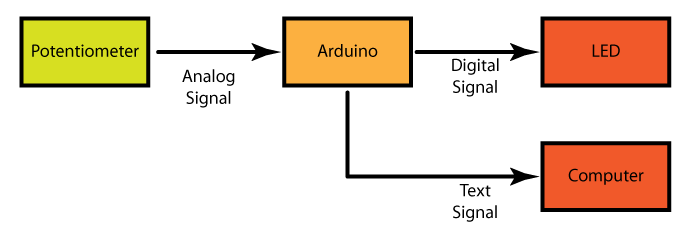
\includegraphics[width=0.5\textwidth]{images/arduino_block_diagram.png}
\caption{Example of Figure 1. Generic Block diagram. Make sure the caption explains the figure.}
\label{fig:block_diag}
\end {center}
\end{figure}

Tables
\begin{flushright} 0.4 Marks \end{flushright}

\begin{table}[!ht] %[H]
\centering
\caption{Connection of Arduino - Force Sensor}
\begin{tabular}{ccccc}
Protoboard adapter pin& Arduino-pin & Use \\ \hline
SIG2   & etc                    & etc          \\

etc &             &      

\end{tabular}
\label{table:connection_diag}
\end{table}

Table \ref{table:connection_diag}, presents the connection between sensor and arduino. 

\section{Results}
\begin{flushright} {\bf Total: } 4.6 Marks \end{flushright}
\begin{flushright} 1 - Breadboard diagram images: 1.2 Marks \end{flushright}
\begin{flushright} 2 - Testing explanation: 1.0 Marks \end{flushright}
\begin{flushright} 3 - Muscular force figures: 2.4 Marks \end{flushright}

Two parts: 1st part testing of user friendly interfaces (LED, LCD) and sensor, 2nd part Arduino integration. \\[0.1in]

{\bf Multicolor LED testing}  
\begin{flushright} 1.2 Marks \end{flushright}
Figure 2. {\it Circuit diagram or Breadboard schematic for multicolor LED}: One Image of the circuit showing the procedure to connect a multicolor LED. You can use any software to produce the circuit or if you choose to show a breadboard image, use Fritzing.
\href{http://fritzing.org/home/}{http://fritzing.org/home/}. 
Describe the image and describe with words what the arduino code does to test the LED.
 Describe the procedure performed to test the multicolor LED (what functions were used, etc.).

\begin{figure}[H]%[!ht]
\begin {center}
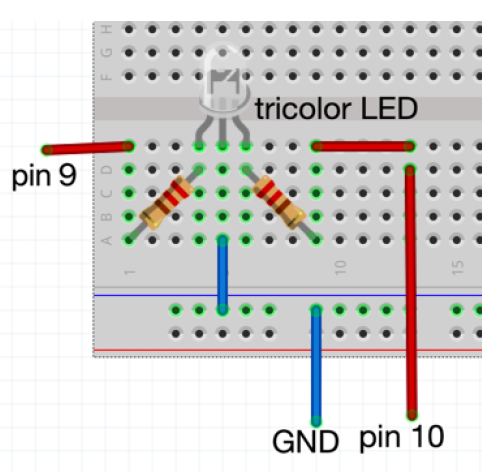
\includegraphics[width=0.35\textwidth]{images/led_fritz.png}
\caption{Example of Figure 2. You can use any software to produce an image of the electric circuit for using a multicolor LED or for breadboard circuits generate your own using Fritzing.  Add Arduino in the Figure.
\href{http://fritzing.org/home/}{http://fritzing.org/home/}}
\label{fig:led_Frit}
\end {center}
\end{figure}

{\bf LCD testing}  
\begin{flushright} 0.5 Marks. \end{flushright}
 Describe the procedure performed to test the LCD screen (what functions were used, etc.).\\[0.1in]

{\bf Sensor testing}  
\begin{flushright} 0.5 Marks \end{flushright}
 Describe the procedure performed to test the sensor (what functions were used, etc.).\\[0.1in]


{\bf Force Measurements} \begin{flushright} 0.8 Marks each figure. \end{flushright} 
Figure 3: {\it Dominant vs non-dominant hand}.
Describe the image and write down differences in magnitude, use quantitative comparison when describing the image(\%,). \\


\begin{figure}[H]
\begin {center}
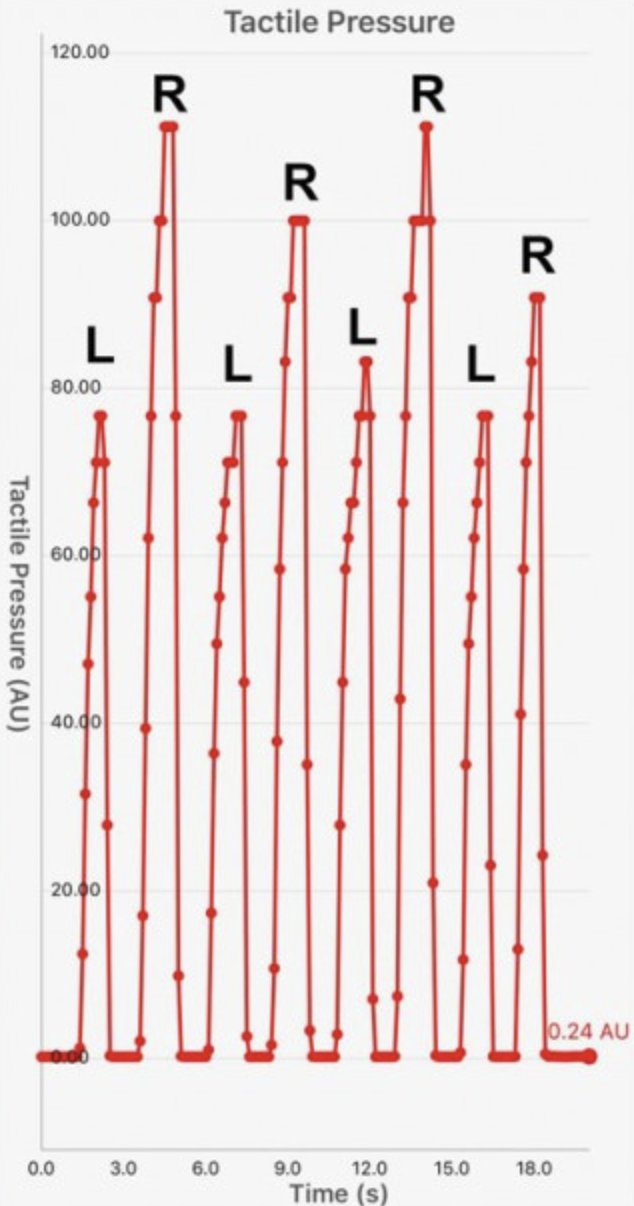
\includegraphics[width=0.25\textwidth,height=2.5333in]{images/dominant_no_dominant.png}
\caption{Example Fig. Make sure the caption explains the figure and all numbers and labels can be clearly read.}
\label{fig:dominant_hand}
\end {center}
\end{figure}

Determine if there is a correlation between hand size and grip strength. Consider factors such as wrist and forearm circumference in relation to grip strength and which muscle complexes are involved in grip strength and pinch strength.
    
Figure 4: {\it Fingers Force}.
Describe the image and write down differences in magnitude, use quantitative comparison when describing the image(\%,). \\
Determine if there is a correlation between fingers size and fingers strength. 

\begin{figure}[H]
\begin {center}
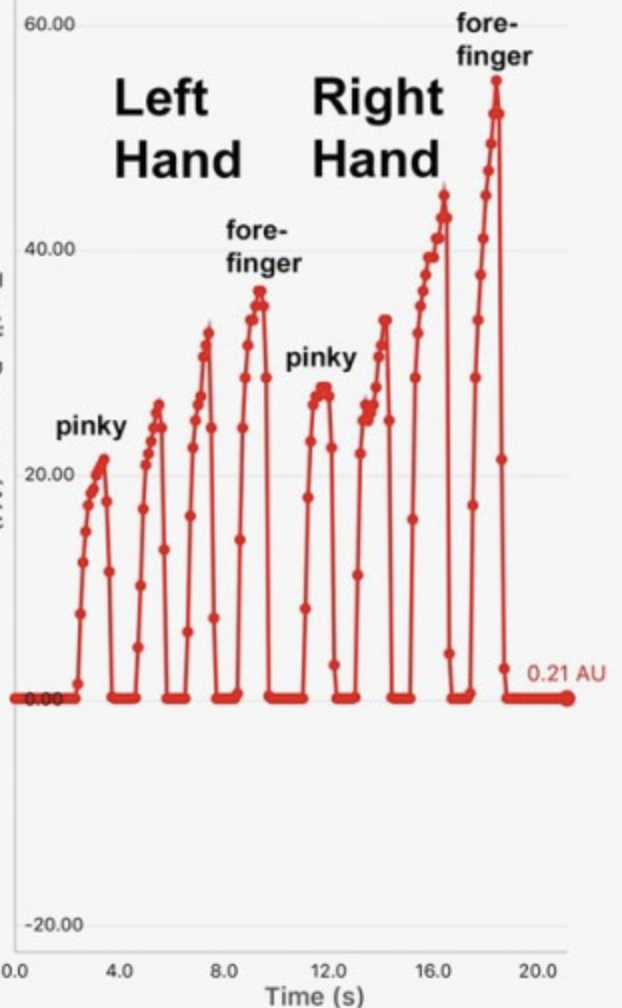
\includegraphics[width=0.25\textwidth,height=2.5333in]{images/fingers_force.png}
\caption{Fingers force. Make sure the caption explains the figure and all numbers and labels can be clearly read.}
\label{fig:fingers_force}
\end {center}
\end{figure}

Figure 5: {\it Fatigue}.
Describe the image and write down differences in magnitude, use quantitative comparison when describing the image(\%,). \\

\begin{figure}[H]
\begin {center}
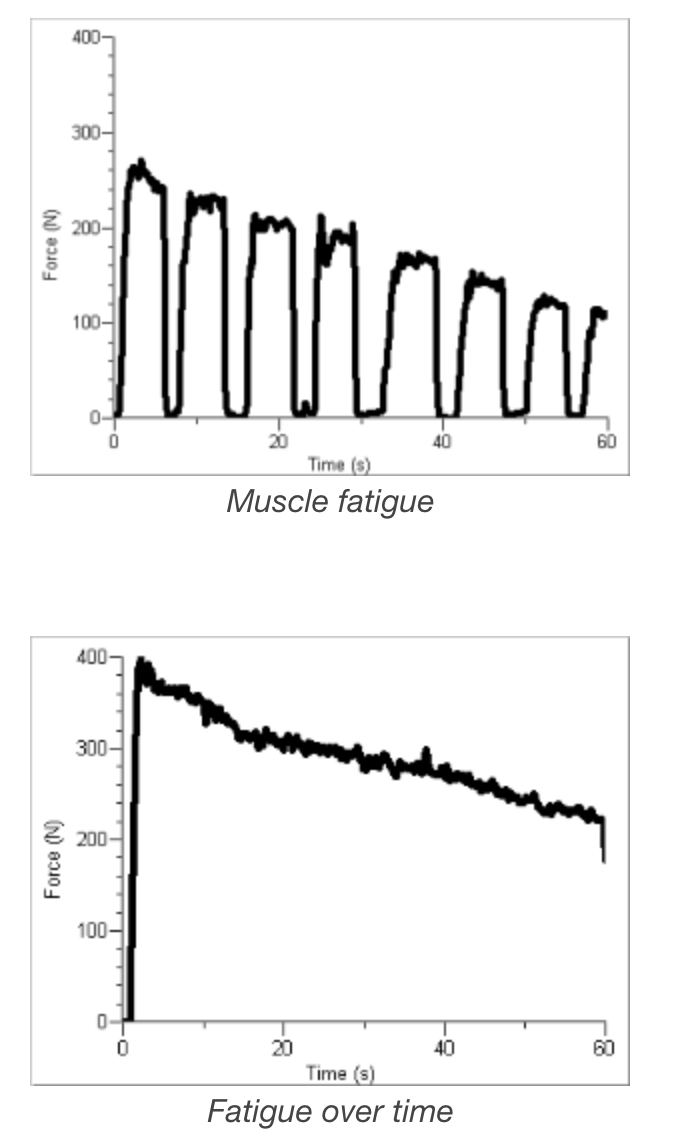
\includegraphics[width=0.45\textwidth,height=2.5333in]{images/fatigue_dynam.png}
\caption{Muscular fatigue can be seen as a drop in force over time. Make sure the caption explains the figure and all numbers and labels can be clearly read.}
\label{fig:fatigue}
\end {center}
\end{figure}

In the data analysis (processing), determine if muscle fatiguing time is similar for all participants and if there is variation between age groupings and gender.  Do this measurements for at least 2 members of the team.\\
    





\section{Discussion and Summary}
\begin{flushright} 1.0 Mark. \end{flushright}

Summarize your findings. Discuss any interesting result related to the materials used or to any claim from the introduction. Discuss your measurements using engineering terms (accuracy, precision, resolution, etc).  Give technical conclusions. Restate the main objectives and how or to what degree they were achieved. Describe some applications of your results and comment any possible recommended future work.



% if have a single appendix:
%\appendix[Proof of the Zonklar Equations]
% or
%\appendix  % for no appendix heading
% do not use \section anymore after \appendix, only \section*
% is possibly needed

% use appendices with more than one appendix
% then use \section to start each appendix
% you must declare a \section before using any
% \subsection or using \label (\appendices by itself
% starts a section numbered zero.)
%


\appendices
\section{Code.}
\begin{flushright} 1.0 Marks. \end{flushright}
Code used.
\begin{itemize}

    \item  Include code used for LED testing, and Force measurement.
    \item  Any substantial addition or interesting change to the code, may give you extra marks.

\end{itemize}
% use section* for acknowledgment

% references section

% can use a bibliography generated by BibTeX as a .bbl file
% BibTeX documentation can be easily obtained at:
% http://mirror.ctan.org/biblio/bibtex/contrib/doc/
% The IEEEtran BibTeX style support page is at:
% http://www.michaelshell.org/tex/ieeetran/bibtex/
%\bibliographystyle{IEEEtran}
% argument is your BibTeX string definitions and bibliography database(s)
%\bibliography{IEEEabrv,../bib/paper}
%
% <OR> manually copy in the resultant .bbl file
% set second argument of \begin to the number of references
% (used to reserve space for the reference number labels box)

%use following command to generate the list of cited references

\printbibliography

\section*{References}
\begin{flushright} 0.2 Mark. \end{flushright}

Example of data book:\\[0.1in]
[1] National Operational Amplifiers Databook. Santa Clara: National Semiconductor
Corporation, 1995 Edition, p. I-54. \\[0.1in]
Example of textbook: \\[0.1in]
[2]M. Young, The Technical Writer’s Handbook. Mill Valley, CA: University Science, 1989.\\[0.1in]
Example of scientific journal paper:\\[0.1in]
[3] J.W. Smith, L.S. Alans and D.K. Jones, “An operational amplifier approach to
active cable modeling”, IEEE Transactions on Modeling, vol. 4, no. 2, 1996, pp.
128-132.\\[0.1in]
Example of conference paper proceedings:\\[0.1in]
[4] J.W. Smith, L.S. Alans and D.K. Jones, “Active cable models for lossy
transmission line circuits”, in Proc. 1995 IEEE Modeling Symposium, 1996, pp.
1086-89.\\[0.1in]

Example of Internet web page:\\[0.1in]
[5] Approximate material properties in isotropic materials. Milpitas, CA: Specialty Engineering Associates, Inc. web site: www.ultrasonic.com, downloaded April 20, 2019.  \\[0.1in]

List and number all bibliographical 
references at the end of your paper in {\bf 9 or 10 point} Times, with 10-point interline spacing. When referenced within the text, enclose the citation number in square brackets, for example [1].\\[0.1in]
Use IEEE format. Cite any external work that you used (data sheets, text books, Wikipedia articles, . . . ). If you get a formula from a Wikipedia article, you must cite the article, giving the title, the URL, and the data you accessed the article as a minimum. If you copy a figure, not only must you cite the article you copied from, but you must give explicit figure credit in the caption for the figure: This image copied from . . . . If you modify a figure or base your figure on one that has been published elsewhere, you still need to give credit in the caption: This image adapted from . . . .
\end{document}


